\chapter{ALGORITHM FOR DAGs}
\label{chap:sup}
 
In this chapter, we propose a new algorithm for Betweenness Centrality specifically for DAGs. 
Consider a Directed Acyclic Graph $G \equiv (V,E)$ where set $V$ contains the vertices and set $E$ contains edges. 
First, we tried to apply the proposed algorithm for tree on DAGs by making making duplicate vertices if a vertex has two or more parents. Converting DAG into a tree with duplicating vertices and then applying the algorithm for trees was less efficient then the existing Brandes' Algorithm. The reason being, multiple shortest path exists in DAG from vertex $s$ to $t$ where $s, t \in V$, which was not the case for trees. And even after converting DAG to tree, the merging of vertices to compute the exact values becomes the bottleneck for the algorithm and no improvement is achieved in terms of execution time.   

So we proposed another algorithm specifically for DAG, which reduces the execution time with respect to Brandes' Algorithm. The outline of proposed algorithm is given in Algorithm 4.
\vspace{1em}
\begin{algorithm}
\caption{Betweenness Centrality of DAG}
Topological sort and Reverse topological sort\;
Backward Propagation()\;
Forward Propagation()\;
\end{algorithm}

\begin{figure}
\centering
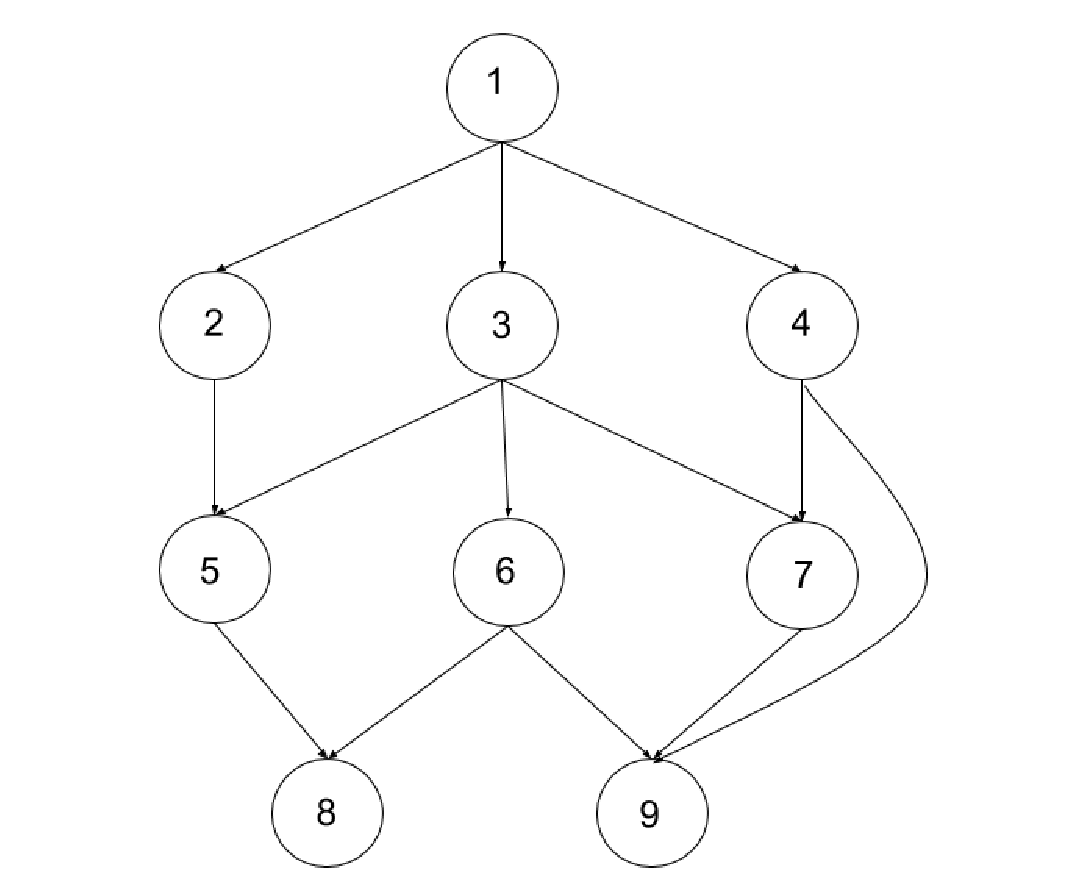
\includegraphics[width=13cm]{images/exampledag.eps}
\caption{Example of DAG}
\label{fig:exdag}
\end{figure}

\section{Backward Propagation Phase}
\begin{algorithm}
%\KwResult{Write here the result }
child $\rightarrow v$, parent $\rightarrow p$ \\
\For{each reachable vertex $t$ from $v$}{
\eIf{$d(v,t) + 1 = d(p,t)$}{
$c(p,t) \leftarrow c(p,t) + 1$\;
}
{
\If{$d(p,t) > d(v,t) + 1$ OR $d(p,t) < 0$}{
$d(p,t) \leftarrow d(v,t) + 1$\;
$c(p,t) \leftarrow c(v,t)$\;
}
}
}
\caption{Backward Propagation}
\end{algorithm}
As mentioned in Algorithm 4, the first step of the proposed algorithm is to compute the topological sort and reverse topological sort of the given graph.

The second step is backward propagation where we use reverse topological sort computed in the first step. The outline of Backward propagation step is given in Algorithm 5. At the end of this step, for any vertex $t$ which is reachable from vertex $v$, the number of shortest paths from $v$ to $t$ and the length of shortest path are stored at vertex $v$. 
For example given in figure 4.1, after backward propagation phase, vertex 1,2,3,4 contains following information: in table 1.


\begin{table}[h!]
\centering
\begin{tabular}{|c|c|c|}
\hline
vertex & length & count \\
\hline
2 & 1 & 1 \\ 
\hline
3 & 1 & 1 \\ 
\hline
4 & 1 & 1 \\ 
\hline
5 & 2 & 2 \\ 
\hline
6 & 2 & 1 \\ 
\hline
7 & 2 & 2 \\ 
\hline
8 & 3 & 3 \\ 
\hline
9 & 2 & 1 \\ 
\hline
\end{tabular}
\caption{Values stored at Vertex 1}
\label{tab:data1}
\end{table}

    \begin{table}[h!]
    \centering
        \begin{tabular}{|c|c|c|}
            \hline
            vertex & length & count \\
            \hline
            5 & 1 & 1 \\ 
            \hline
            8 & 1 & 1 \\ 
            \hline
        \end{tabular}
    \caption{Values stored at Vertex 2}
    \label{tab:data2}
    \end{table}


\begin{table}[h!]
\centering
\begin{tabular}{|c|c|c|}
\hline
vertex & length & count \\
\hline
5 & 1 & 1 \\ 
\hline
6 & 1 & 1 \\ 
\hline
7 & 1 & 1 \\ 
\hline
8 & 2 & 2 \\ 
\hline
9 & 2 & 2 \\ 
\hline
\end{tabular}
\caption{Values stored at Vertex 3}
\label{tab:data3}
\end{table}




\begin{table}[h!]
\centering
\begin{tabular}{|c|c|c|}
\hline
vertex & length & count \\
\hline
7 & 1 & 1 \\ 
\hline
9 & 1 & 1 \\ 
\hline
\end{tabular}
\caption{Values stored at Vertex 4}
\label{tab:data4}
\end{table}




In reverse topological sort order, any vertex $t$ pushes the information it possess to all its parents. Reverse topological sort order is used because we are pushing information from a child to a parent so the child's information should be computed first and it should not change, otherwise the changed value propagates to the other vertices in case the order is not considered. 

A vertex $u$ updates the values at its parent $w$.
While updating values for vertex $v$ such that shortest path length from $u$ to $v$ is $x$ with count $c1$ then based on values present at vertex $w$ three cases arises:
\begin{enumerate}
\item  $x + 1 >$ path length from $w$ to $v$
\item  $x + 1$ = path length from $w$ to $v$
\item  $x + 1 <$ path length from $w$ to $v$
\end{enumerate}
\vspace{-2.0em}
\subsection{CASE 1}
\vspace{-1.0em}
Since a shorter path exists through other vertex, $u$ doesn't updates values for $v$ at vertex $w$.
For example given in figure 4.1, vertex '3' tries to update the value at its parent vertex '1' for vertex '9'. The shortest path length from vertex '3' to vertex '9' is  '2'. Whereas Vertex '4' has already updated its values at vertex '1'. Hence vertex '1' already contains a shortest path to  vertex '9' of length 2 i.e 1-4-9. When 3 tries to update value 3 as a path length to vertex '9' at vertex '1', it won't update because there already exists a shorter path through some other vertex and in this case vertex '4'. 

\subsection{CASE 2}
Since there exists shorter paths through other vertices, so $u$ only increments the existing number of paths from vertex $w$ to $v$ by $c1$.
In figure 4.1, vertex '3' tries to update the value at its parent vertex '1' for vertex '7'. The shortest path length from vertex '3' to vertex '7' is  '1'. Whereas Vertex '4' has already updated its values at vertex '1'. Hence vertex '1' already contains a shortest path to vertex '7' of length 2 with number of paths as 1, i.e 1-7-9.
So, vertex '3' increments count of number of paths from vertex '1' to vertex '9' by the number of shortest path from vertex '3' to vertex '9' which is 1. Thus vertex '3' has a shortest path of length 2 and number of such paths are 2.

\subsection{CASE 3}
Since the shortest path from vertex $w$ to $v$ doesn't exist or is of length greater than the path through $u$, so $u$ updates the shortest path length as $x + 1$ and also the number of such paths as $c1$.
In figure 4.1, vertex '5' updates vertex '3' for vertex '8' as path length 1 and number of such paths as 1 since vertex '3' doesn't has any path to vertex '8' before any updates by vertex '6'. 

After backward propagation phase, any vertex $v$ will have total number of shortest paths to each reachable vertex from $v$ and their path length.
\section{Forward Propagation Phase}

\begin{algorithm}
%\KwResult{Write here the result }
$bc[v] \leftarrow$ 0, $v \in V$\;
\For{each parent $p$ of vertex $v$}{
\For{each reachable vertex $t$ from $v$}{
\If{$d(v,t) + 1 = d(p,t)$}{
$\Delta_{vt} \leftarrow c(v,t)/c(p,t)$\;
$\delta{vt} \leftarrow \delta{vt} + \Delta_{vt}*(1 + \delta{pt})$\;
$bc[v] \leftarrow bc[v] + \Delta_{vt}*(1 + \delta{pt})$\; 
}
}
}
\caption{Forward Propagation}
\end{algorithm}

In Algorithm 6, $d(v,t)$ is shortest distance calculated in second step from $v$ to $t$ whereas, $c(v,t)$ is count of shortest path from $v$ to $t$. $\Delta_{vt}$ is ratio of number of shortest paths to $t$ which passes through $v$. 
The third step is to calculate Betweenness Centrality in the topological sorted order of vertices computed in the first step. For each parent $p$ of vertex $v$, we check whether there is shortest path to any node $t$ reachable from $v$ such that distance from $p$ is (distance from $v$ + 1). If such a path exists then we calculate Betweenness Centrality which is given in Algorithm 6. 


\section{Summary}
The betweenness centrality values are calculated correctly with reduced execution time with respect to Brandes' Algorithm.
The issue with this algorithm is that it requires a huge amount of space since we store count and distance for each reachable vertex $t$ from $v$ at vertex $v$.